% Based on a template created by João Alegria (https://github.com/joao-alegria)
%  and Filipe Pires (https://github.com/FilipePires98)

\documentclass[12pt]{article}

\usepackage[english]{babel}
\usepackage[utf8x]{inputenc}

\usepackage{float}
\usepackage{hyperref}
\usepackage{times}
\usepackage{url}

% Images
\usepackage{graphicx}
\graphicspath{{images/}}

% Page dimensions
\topmargin -1.0cm
\oddsidemargin 0.0cm
\textwidth 16cm
\textheight 23cm
\footskip 1.0cm

% TITLE PAGE CONTENT BEGIN

\title{Assignmnet 3}

\author{
    André Pedrosa [85098], João Abílio [84732]\\
    \\
    Recuperação de informação\\
    \normalsize{Departamento de Eletrónica, Telecomunicações e Informática}\\
    \normalsize{Universidade de Aveiro}\\
}

\date{13 de dezembro de 2019}

% TITLE PAGE CONTENT END

\begin{document}

\baselineskip18pt

\maketitle

\section*{1. Introdução}
Este relatório apresenta uma explicação do trabalho desenvolvido
para o terceiro assignment da disciplina "Recuperação de Informação",
explicando as decisões tomadas e o funcionamento da solução.

Esta terceira entrega tem como objetivo fazer incrementos à entrega
anterior de maneira a criar uma pipeline que permitia fazer
perquisa sobre o index invertido criado na entrega anterior.

No fim serão apresentados as métricas de eficiência e avaliação dos
resultados devolvidos pelo motor de pesquisa desenvolvido.

Devido ao elevado número de classes criadas, o diagrama de classes
vai ser dividido em vários que vão sendo apresentados ao longo do
relatório. Estes diagramas foram gerados através do IDEA IntelliJ,
consequentemente em anexo é disponibilizada a legenda da convenção
usada.

\section*{2. Data Flow}
\begin{figure}[h]
  \center
  \includegraphics[width=\linewidth]{newsequenceDiagram.png}
  \caption{Diagrama de sequência da solução}
  \label{fig:dataflow}
\end{figure}

O data flow da nossa solução, de modo geral não sofreu grandes
alterações, apenas migramos o código de execução da pipeline de
indexação para uma classe separada, em vez de ser definida na
classe Main.

Na figura \ref{fig:dataflow} está representado sequência de execução
da nossa solução, onde as setas azuis significam que a classe origem
executa um método da classe destino e as setas vermelhas significam
que a classe origem cria a classe destino. Deixando de parte as classes
que têm uma seta vermelha a apontar para si, todas as classes são
instanciadas na classe Main. Na figura existem várias classes em que é
apresentado a classe base e a sua implementação, isto pois algumas
classes base apresentam métodos {\it final} que chamam depois métodos
abstratos que devem estar definidos em classes de descendentes (padrão
Template Method).

\section*{3. Packages}
\begin{figure}[H]
  \center
  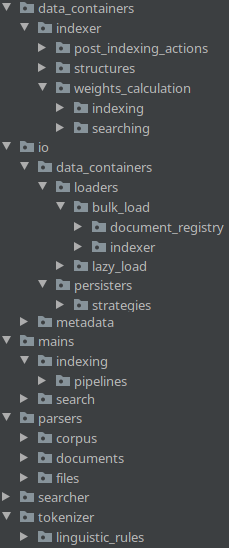
\includegraphics[width=6cm]{packages_all.png}
  \caption{Árvore de packages da solução}
\end{figure}

Nesta secção vão ser apresentadas as alterações feitas a cada package
relativamente à entrega anterior.

\section*{3.1. tokenizer}
\begin{figure}[H]
  \center
  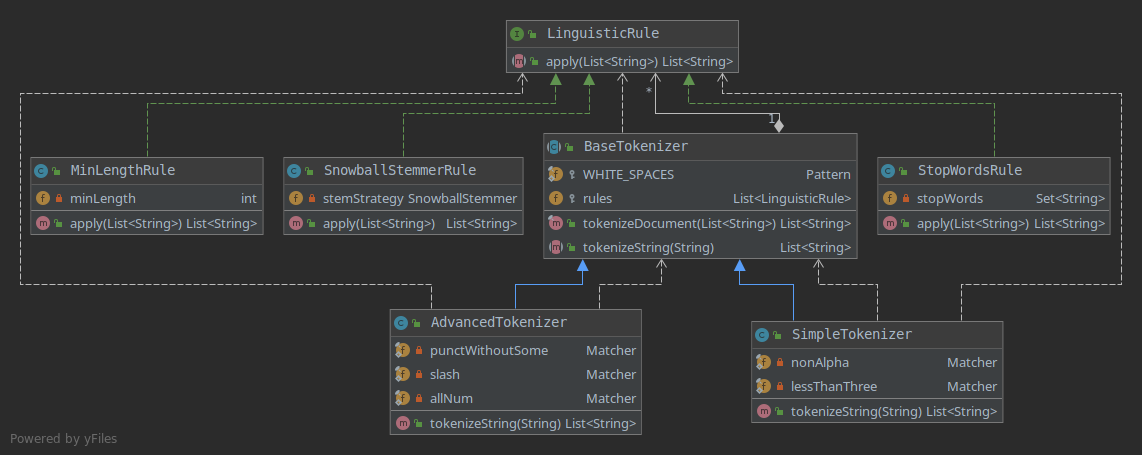
\includegraphics[width=\linewidth]{packages_tokenizer.png}
  \caption{Diagrama de classes do package \it tokenizer}
\end{figure}

Este package também não sofreu alterações relativamente à
entrega anterior.

\section*{3.2. parsers}
\begin{figure}[H]
  \center
  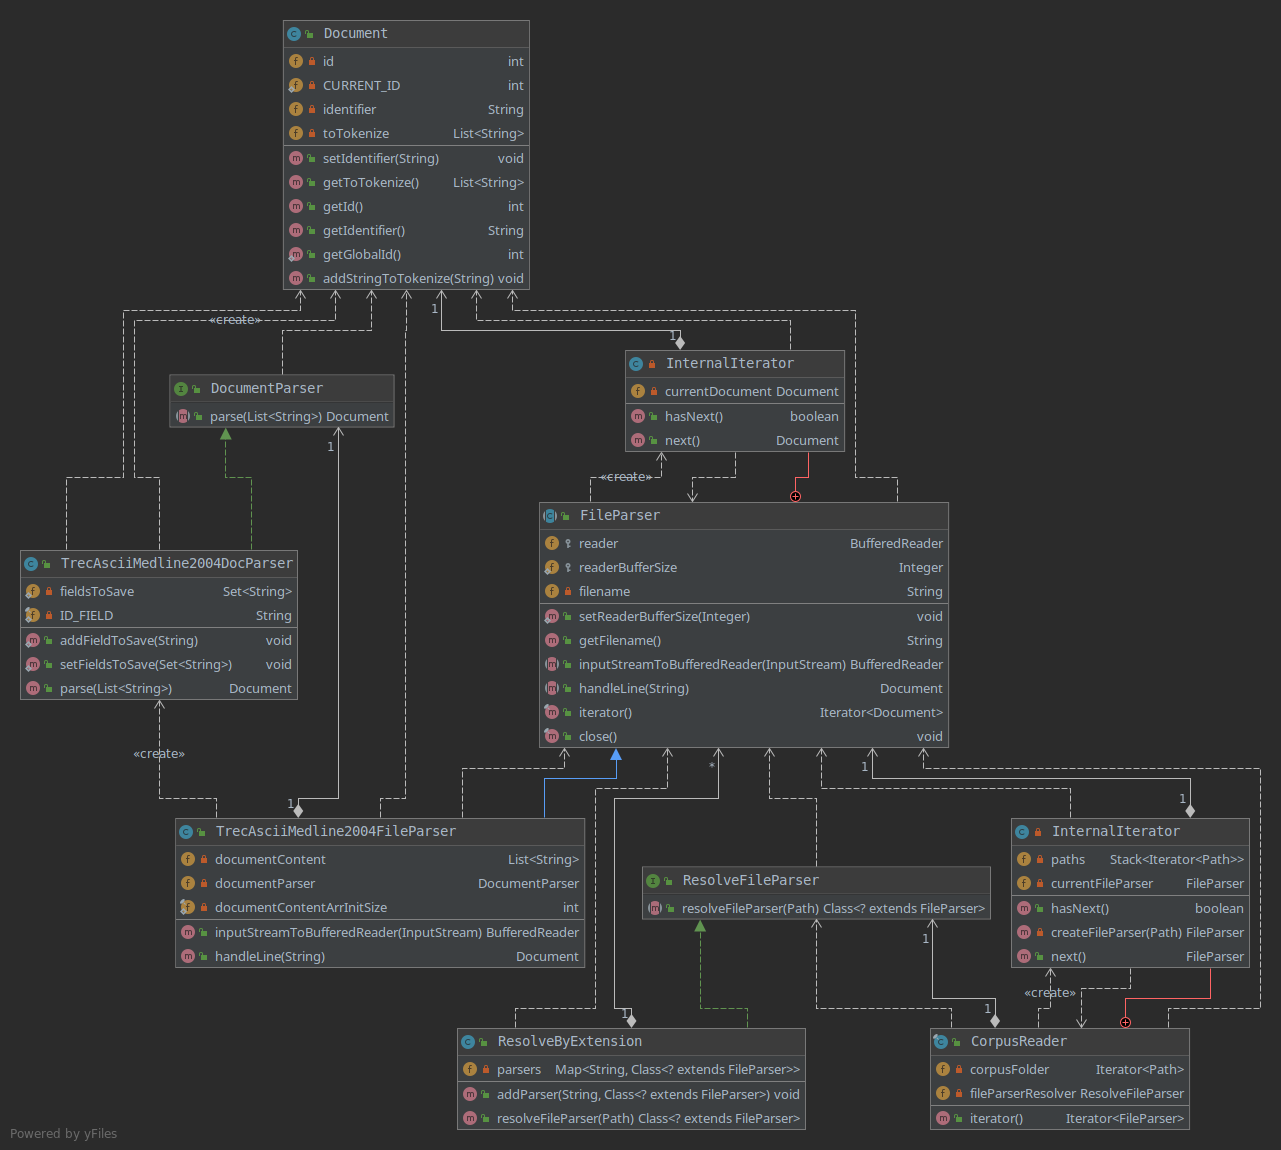
\includegraphics[width=\linewidth]{packages_parsers}
  \caption{Diagrama de classes do package \it parsers}
\end{figure}

Este package não sofreu grandes alterações relativamente à entrega
anterior, apenas foi alterado o tipo de dados do identificador
original de cada documento de {\it String} para {\it int}.

\section*{3.3. data\_containers}
Na entrega anterior tanto o inverted index como o document registry
estavam presentes na mesma classe, Indexer.
Isto trazia alguns problemas para a pipeline de pesquisa pois quando
o inverted index era carregado o respetivo document registry devia
também de ser carregado.
No entanto um termo pode ter um documento de id 1, que foi o primeiro
a ser indexado, e outro com id 4.000.000, um dos últimos a serem
indexados.
Isto implicava consultar diferentes segmentos do document registry já
em disco na altura de indexação, isto supondo que não conseguimos ter
todos em memória.

Com isto em consideração separamos o document registry e o indexer em
duas classes, o Indexer que contem o inverted index (Map) e o
DocumentRegistry que contem a tradução entre o nosso identificador
interno com o identificador original (Map).
É de realçar que estas classes apenas serão usadas em tempo de
indexação.

Na entrega anterior quem tinha a responsabilidade de atribuir novos
ids internos aos documentos que iam sendo indexados era a classe
Document do package parsers.
Nesta entrega esta responsabilidade foi mudada para a nova classe
DocumentRegistry.

\section*{3.3.1. data\_containers.indexer}
\begin{figure}[h]
  \center
  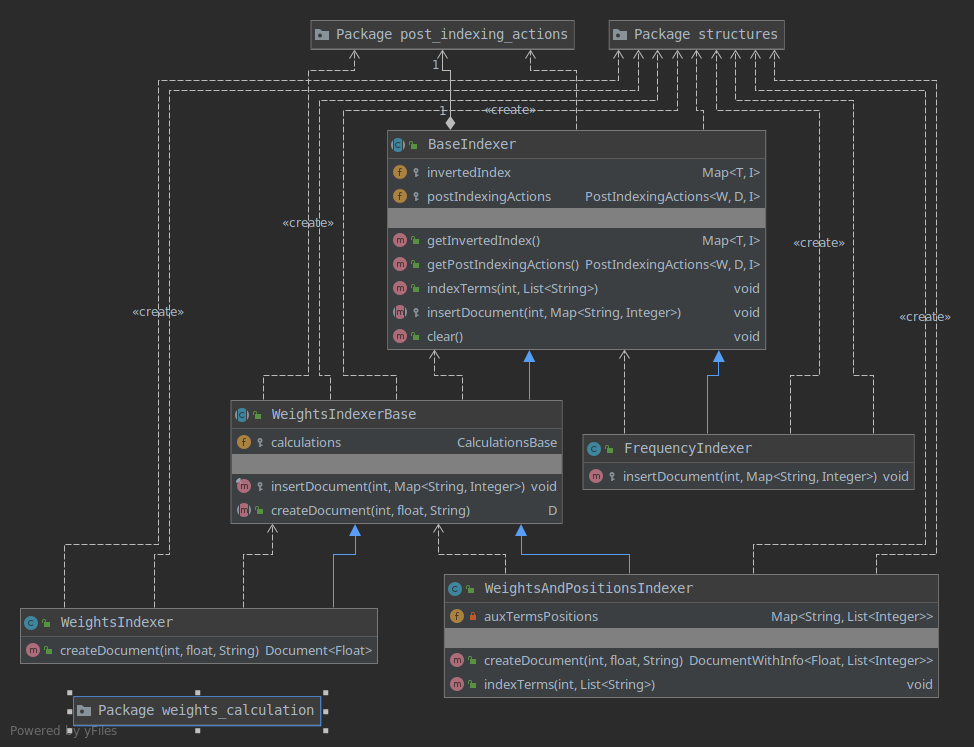
\includegraphics[width=\linewidth]{packages_data_containers_indexer.png}
  \caption{Diagrama de classes do package \it
    data\_containers.indexer}
\end{figure}

Este package sofreu algumas alterações, no entanto as alterações
foram feitas mais ao nível dos sub packages o que levou a adaptações
depois das classes presentes na root deste package.

\section*{3.3.1.1 data\_containers.indexer.post\_indexing\_actions}
\begin{figure}[h]
  \center
   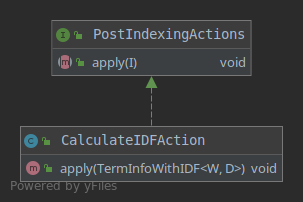
\includegraphics[width=6cm]{packages_data_containers_indexer_post_indexing_actions.png}
  \caption{Diagrama de classes do package \it
    data\_containers.indexer}
\end{figure}

Como na entrega anterior o pesos dos documentos estavam a ser mal
calculados, estando a ser calculados por termos em vez de por
documentos, a {\it post indexing action} criada agora apenas calcula
o idf dos termos, que apenas pode ser calculado no final do processo
de indexação.

\section*{3.3.1.2 data\_containers.indexer.structures}
\begin{figure}[H]
  \center
   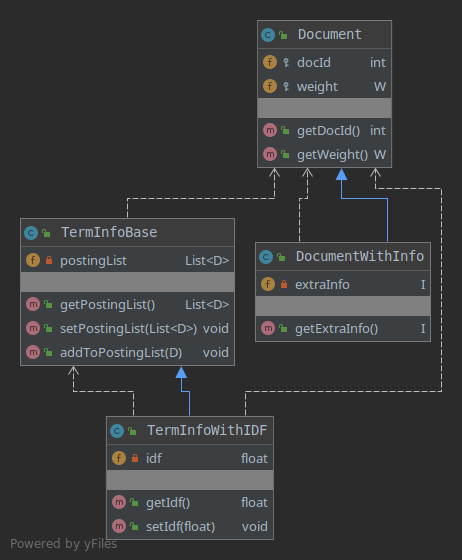
\includegraphics[width=7cm]{packages_data_containers_indexer_structures.png}
  \caption{Diagrama de classes do package \it
    data\_containers.indexer.structure}
\end{figure}

Neste package temos as estruturas que vão ser usadas para armazenar a
informação relativa aos documentos indexados no inverted index.

Este package sofreu algumas alterações devido ao facto de em entregas
anteriores objetos com informação serem usados como chave do inverted
index e esta ser necessária posteriormente na fase de pesquisa. Mais
concretamente falamos do objeto Term em que usávamos o termo para
gerar o hashcode e também para comprar objetos Term para depois ser
inserido em HashMaps ou ordenados respetivamente.

Um exemplo de informação extra que era guardada no objeto Term era o
idf de um termo. No entanto para obter este teríamos de percorrer
todas as chaves do HashMap até encontrar aquela que tinha o termo
igual ao que queríamos obter o idf. Isto é uma operação $O(n)$, ou
seja, estávamos a perder o tempo constante de acesso a um HashMap.

De maneira a corrigir o problema apenas definimos objetos para os
valores associados a um termo indexado, ou seja, os valores de um
HashMap. Estes valores são do tipo {\it TermInfoBase} que contêm
sempre uma posting list de documentos. Cada documento tem sempre um
id e um peso associado. Podem ainda existir subclasses da classe {\it
TermInfoBase} que podem ter outras informações como o idf (objeto
{\it TermInfoWithIdf}) e os documentos podem também ter outras
informações associadas como as posições (objecto {\it
DocumentWithInfo}).

\section*{3.3.1.3 data\_containers.indexer.weights\_calculation}
\begin{figure}[H]
  \center
   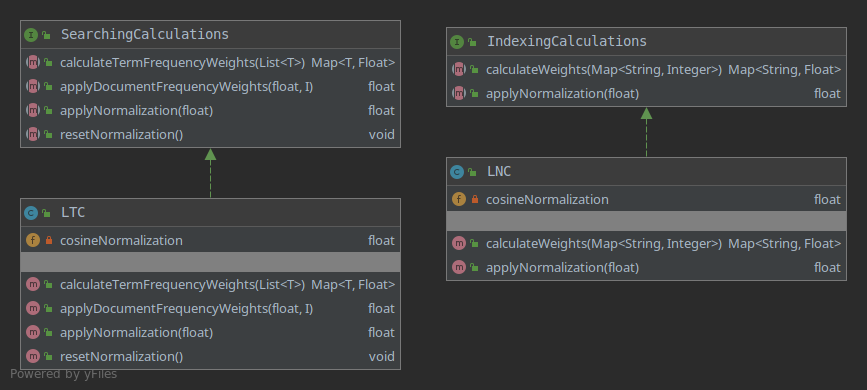
\includegraphics[width=15cm]{packages_data_containers_indexer_weights_calculation.png}
  \caption{Diagrama de classes do package \it
    data\_containers.indexer.weights\_calculations}
\end{figure}

Este package possibilita o calculo de diferentes variantes de pesos a
serem usados durante o processo de indexação ou pesquisa.
Para esta entrega apenas desenvolvemos as classes necessárias para
calcular a variante {\it lnc.ltc}.

\section*{3.4. io}

Na entrega anterior, para sabermos quais os termos presentes num
determinado ficheiro de indexer ou document registry, os nomes destes
ficheiros continham a chave da primeira entry guardada nesse.
Ou seja, se tivéssemos dois ficheiros um com nome {\it aaa} e outro
{\it bbb} sabíamos que o termo {\it abc} estava no ficheiro {\it
aaa}.

No entanto nesta entrega mudamos a nossa estratégia e passamos a
guardar estes metadados num ficheiro separado.

Como este package passou a não guardar só estrutura relativas ao
indexer migramos o package para a root do projeto.

\section*{3.4.1 io.metadata}
\begin{figure}[H]
  \center
   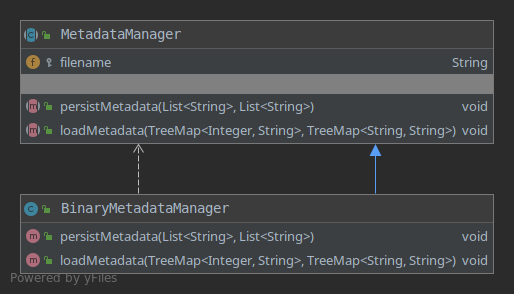
\includegraphics[width=8cm]{packages_io_metadata.png}
  \caption{Diagrama de classes do package \it
    io.metadata}
\end{figure}

Neste package encontramos diferentes estratégias de gerir em disco os
meta dados do sistema de recuperação de informação.
O meta dados têm a associação entre a chave da primeira entry guarda
em cada ficheiro de indexer (chave é o termo) e document registry
(chave é o nosso id interno) e o número total de documentos indexados
(presente na classe DocumentRegistry).

De maneira a sabermos rapidamente em que ficheiro um certo termo ou
id interno está durante a fase de procura, usamos um TreeMap para
guardar as associações referidas, em que as chaves são as tais
primeiras chaves guardadas num ficheiro e o valor é o nome do
ficheiro em disco onde está guardo.
Fazemos depois uso do método {\it floor} desta classe que nos dá a
maior chave que é menor ou igual à chave que procuramos.
Ou seja, se quisermos traduzir um documento com id 1000 e tivermos
dois ficheiros um em que o primeiro id que guarda é o 0 e outro
1.000.000 ao chamar o método {\it floor} com o argumento 1000 irá
devolver o nome do ficheiro em que o primeiro id é 0.

\section*{3.4.2 io.data\_containers}

Este package foi originado do package {\it indexer.io} da entrega anterior,
em que contêm o loaders e persister para os diferentes data
containers, indexer e document registry.

\section*{3.4.2.1 io.data\_containers.loaders}
\begin{figure}[H]
  \center
   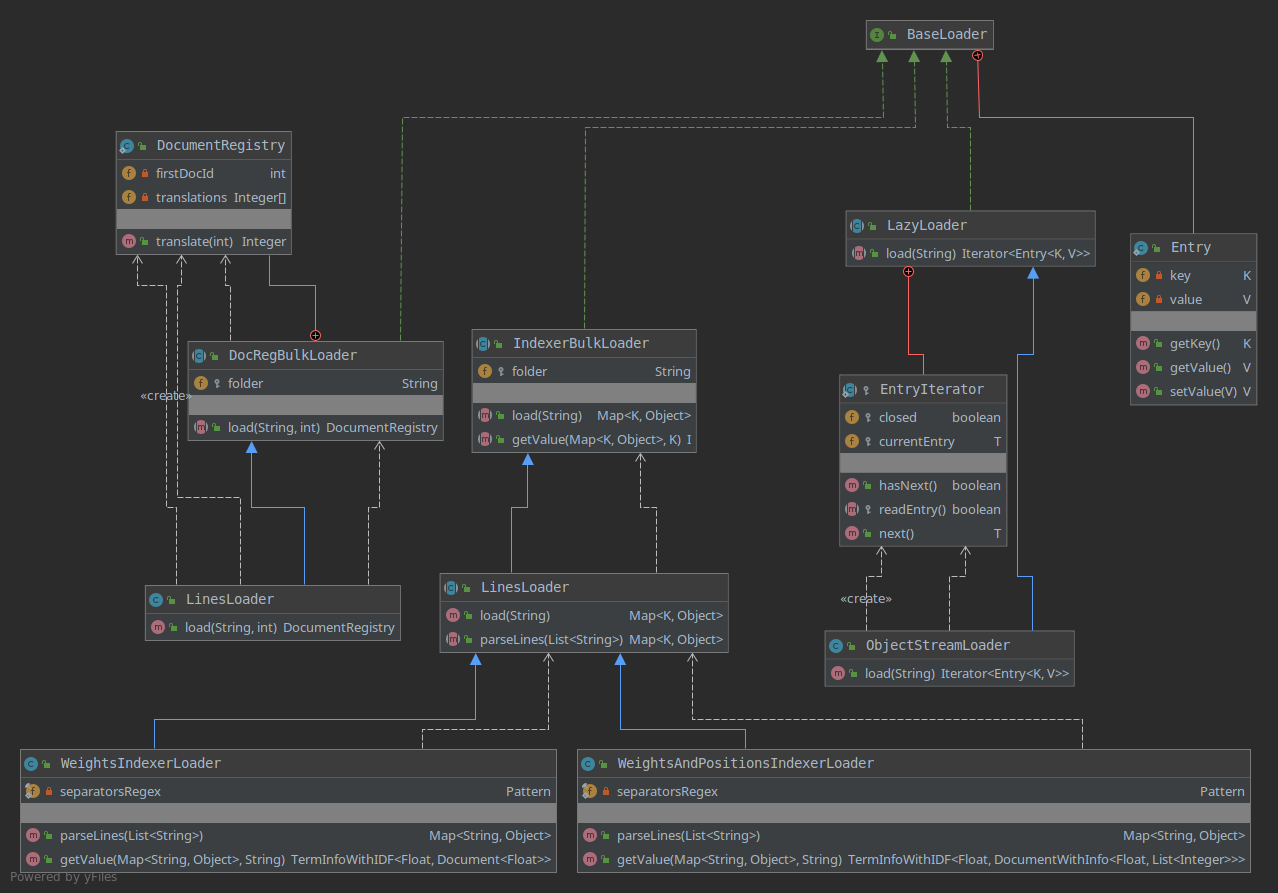
\includegraphics[width=\linewidth]{packages_io_data_containers_loaders.png}
  \caption{Diagrama de classes do package \it
    io.data\_containers.loaders}
\end{figure}

Na entrega anterior apenas tínhamos desenvolvido laoders do tipo {\it
lazy}, ou seja, era carregado uma entry de cada vez do ficheiro. Isto
foi feito para evitar carregar todas as entries para memória e ao
mesmo tempo fazer merge dos vários ficheiros temporários criados pela
pipeline SPIMI.

Neste entrega desenvolvemos também loaders to tipo {\it bulk}, em que
carregam todo o conteúdo para memória de uma vez.

No caso dos indexers, ao carregar para memória é necessário
transformar o dados em disco em objetos, contudo durante a pipeline
de pesquisa podemos não vir a aceder a todas as posting lists de um
ficheiro indexer que carregamos, ou seja, estaríamos a desperdiçar
tempo de computação.
Para evitar isto, os {\it bulk} loader de indexers carregam o
conteudo para um mapa em que a chave é o termo e o valor pode ser o
conteúdo ainda por processar lido do ficheiro ou já processado, isto
é, usamos o tipo Object.

Relativamente ao document registry, como não tem um overhead tão
grande de inicialização de objetos como o indexer, simplesmente
transformamos os identificadores em inteiros, guardamos num array
continuo e tem de ser dada ao loader a informação de a qual document
id interno o primeiro identificador diz respeito ($firstDocId$).
Sabendo isto caso o utilizador queira saber qual a tradução do
documento com document id $y$ simplesmente acedemos à posição $y –
firstDocId$. Caso o resultado da subtração anterior dê um índice fora
do array de identificadores é devolvido {\it null}.


\section*{3.4.2.2 io.data\_containers.persisters}
\begin{figure}[H]
  \center
   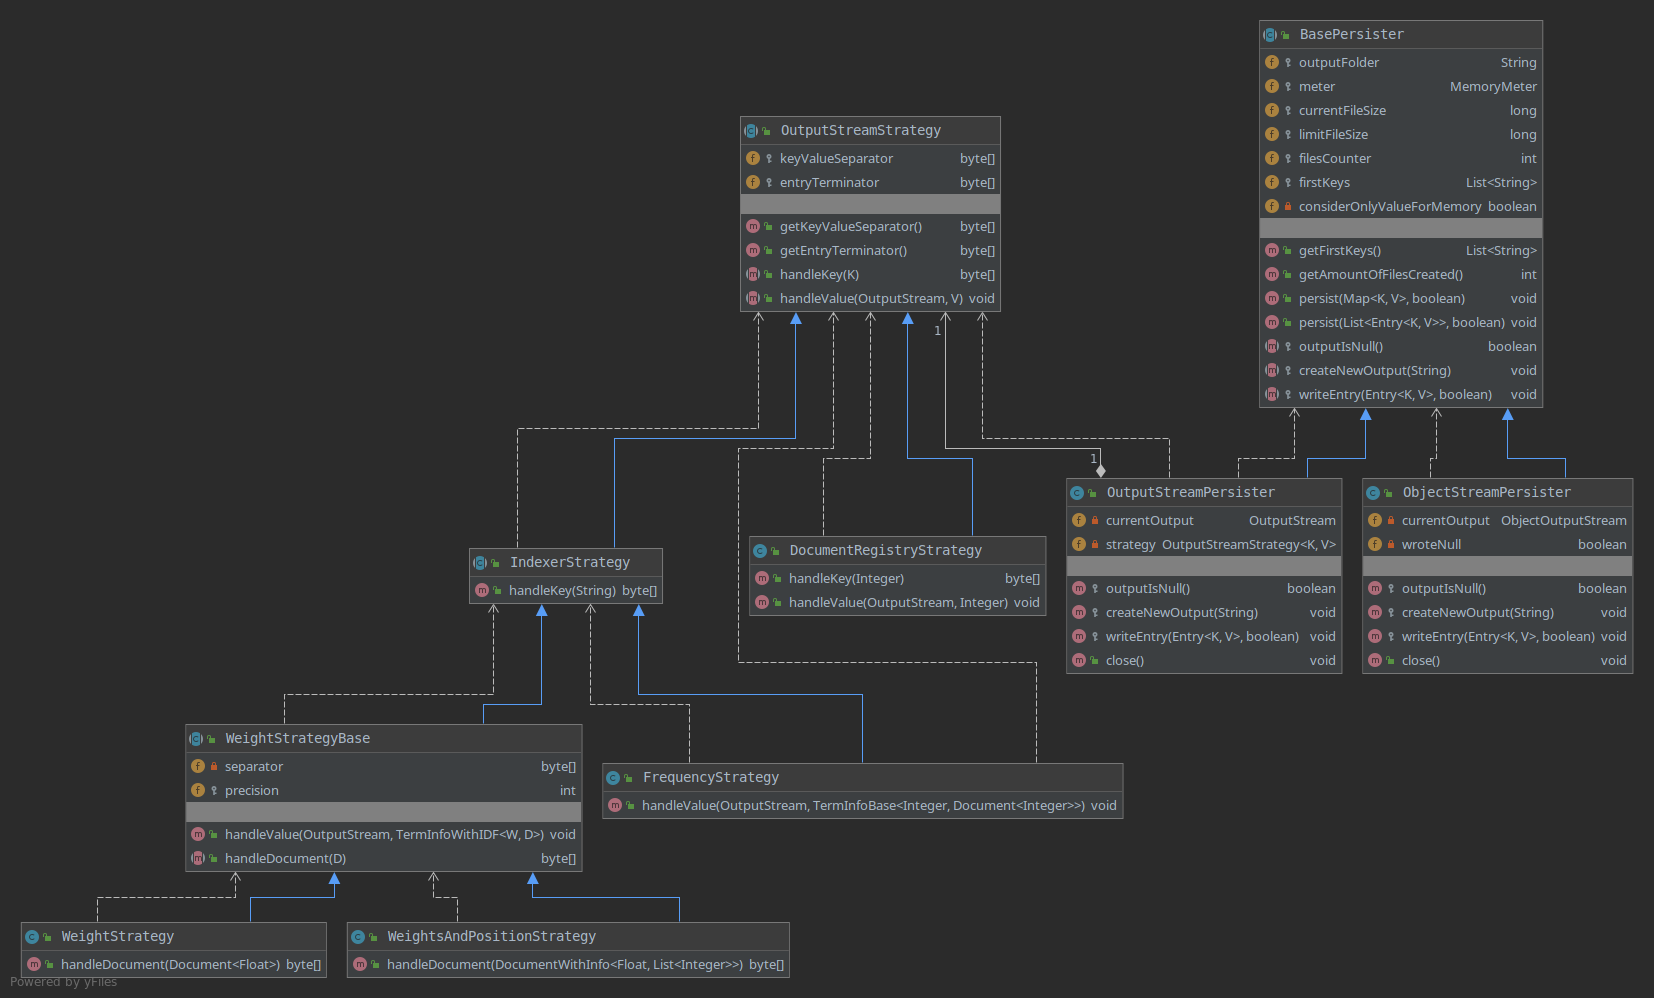
\includegraphics[width=\linewidth]{packages_io_data_containers_persisters.png}
  \caption{Diagrama de classes do package \it
    io.data\_containers.persisters}
\end{figure}

Os persisters, relativamente à entrega anterior, simplesmente
receberam uma alteração associada à maneira como deve ser feita a
segmentação dos indexers e do document registry em disco.
Na entrega anterior o limite estava imposto no número de entries em
cada ficheiro, todavia com isto não sabíamos com certeza o tamanho de
cada ficheiro tanto em disco como em memória.

Para corrigir isto usámos um biblioteca exterior \footnote{Java Agent
for Memory Measurements - https://github.com/jbellis/jamm/} que
percorre a árvore de objetos de um objeto e devolve uma aproximação
em bytes do seu tamanho.
Isto permite-nos depois fazer load para memória de ficheiros inteiro
de indexers ou document registry durante a pesquisa e fazer um gestão
mais informada do que podemos manter em memória durante esse
processo.

\section*{3.5. searcher}
\begin{figure}[H]
  \center
   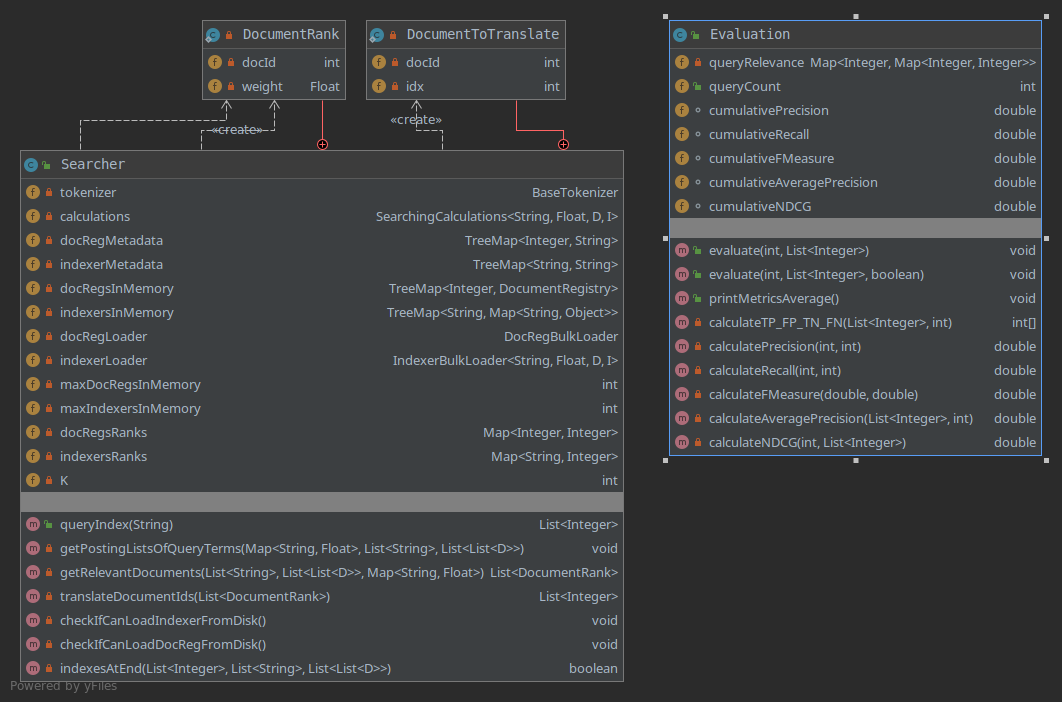
\includegraphics[width=\linewidth]{packages_searcher.png}
  \caption{Diagrama de classes do package \it searcher}
\end{figure}

Aqui está presente a classe que implementa o método de ranked
retrieval, Searcher.
Esta tem um método publico onde recebe uma query, que começa por
fazer a tokenização da query e calcula as term frequencies dos termos
da query segundo a classe de calculo de pesos
(SearchingCalculations).
É de realçar que não estamos a assumir a frequência dos termos da
query a 1, no entanto isto podia ser facilmente alterado criando uma
classe descendente de SearchingCalculations que o faz.

Antes de passar a explicar o que se segue, explicamos primeiro como
gerimos em memória os vários segmentos do indexer e do document
registry.

Primeiro, tanto os indexers como os document registries têm um número
máximo de segmentos que podem se mantidos em memória.

Segundo, a certa altura vamos ter de limpar alguns segmentos em
memória para carregar outros pois não encontramos em memória o termo
ou identificador que procuramos.
Para evitar estar a limpar segmentos que possam ser reutilizáveis
posteriormente, mantemos, para cada segmento, o número de vezes que
foi consultado e deu uma resposta com sucesso (indexersRanks e
docRegsRanks).
Quando temos de limpar a memória retiramos a metade de segmentos que
teve menor consultas (métodos checkIfCanLoadIndexerFromDisk e
checkIfCanLoadDocRegFromDisk).

Passando então para a próxima fase de procura onde temos de obter as
posting lists dos termos da query.
De maneira a tentar reduzir o número de vezes que carregamos de disco
diferentes segmentos ordenamos os termos e assim termos a garantia
que se dois termos da query estiverem no mesmo segmento, este apenas
só é carregado uma vez.
Por exemplo se os termos da query forem {\it a, aa, z} e supondo que
só podemos ter um segmento em memória e que os termos {\it a} e {\it
aa} estão no mesmo segmento e o {\it z} noutro, ao processar os
termos na ordem {\it a, z, aa} iria carregar o segmento do {\it a},
limpa-lo da memória, carregar o do {\it z} e ira carregar novamente o
primeiro segmento.

Com as posting lists dos termos da query em memória, passamos agora a
calcular os pesos para cada documento indexado.
Para isto tiramos partido das nossas posting lists estarem ordenadas
por ordem crescente de document id o que nos permite encontrar
facilmente o mesmo documento nas diferentes posting lists.
Para fazermos isto cada posting list tem um índice associado. Segundo
estes índices obtemos os documentos das posting lists que têm os
document ids mais baixos e comuns, ou seja, relativos ao mesmo
documento.
Cada um destes documentos tem o peso do respetivo termo da query no
documento a que estão associado, que é o mesmo pois têm o mesmo
document id.
Depois de ser calculado o peso para o documento adiciona-se a
associação do peso e document id numa lista de documentos relevantes
e avançam-se os índices das posting lists de onde foram consultados
os documentos usados para calcular o peso do documento que acabou de
ser adicionado à lista de documentos relevantes.

\begin{figure}[H]
  \center
   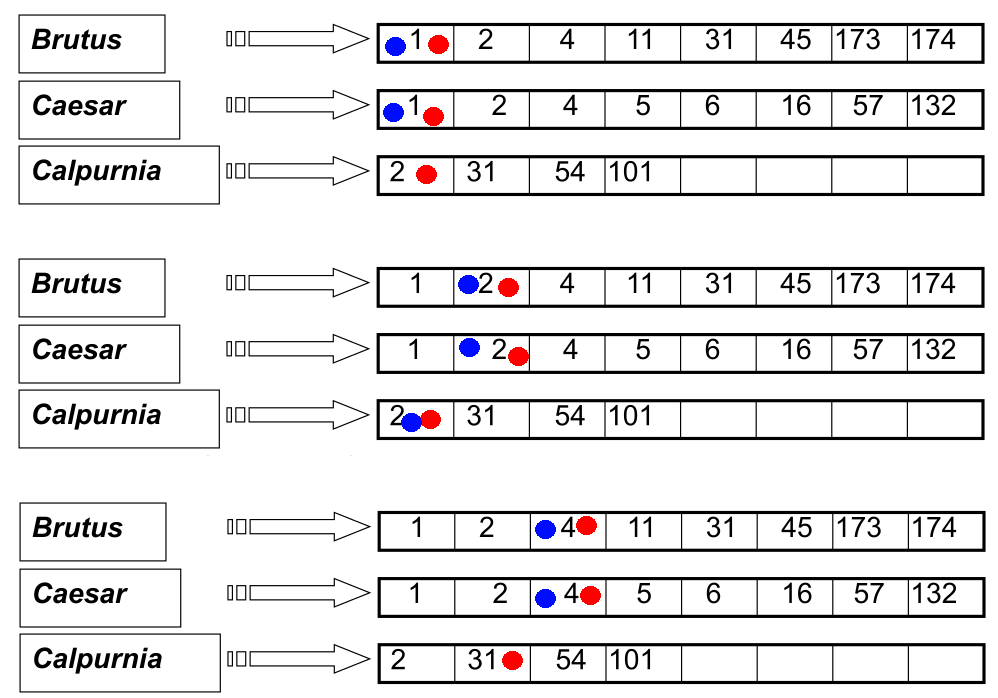
\includegraphics[width=\linewidth]{merge_algorithm.png}
  \caption{Ilustração de como percorridas as posting lists para calcular os pesos para cada documento}
  \label{fig:merge_algorithm}
\end{figure}

Na figura \ref{fig:merge_algorithm} podemos ver como são percorridas
as posting lists de maneira a obter os documentos que referenciam o
mesmo documento, onde as bolas vermelhas indicam onde os índices da
respetiva posting list se encontram e as bolas azuis indicam quais os
documentos que vão ser usados para calcular o peso do documento a
que estão associados.

Depois disto os documentos relevantes são ordenados de forma
decrescente de peso e são retornados os primeiros K documentos.

No entanto o id destes documentos tem ainda de ser traduzido para o
seu identificador original.
Para isso é feito o mesmo processo em termos de consulta de segmentos
e gestão de memória que foi feita com o index mas neste caso para o
document registry.

Neste package encontra-se também a classe responsável por calcular as
várias métricas de avaliação, em que compara os resultados devolvidos
pelo Searcher com um conhecido {\it golden standard}.

\section*{3.6. mains}
\begin{figure}[H]
  \center
   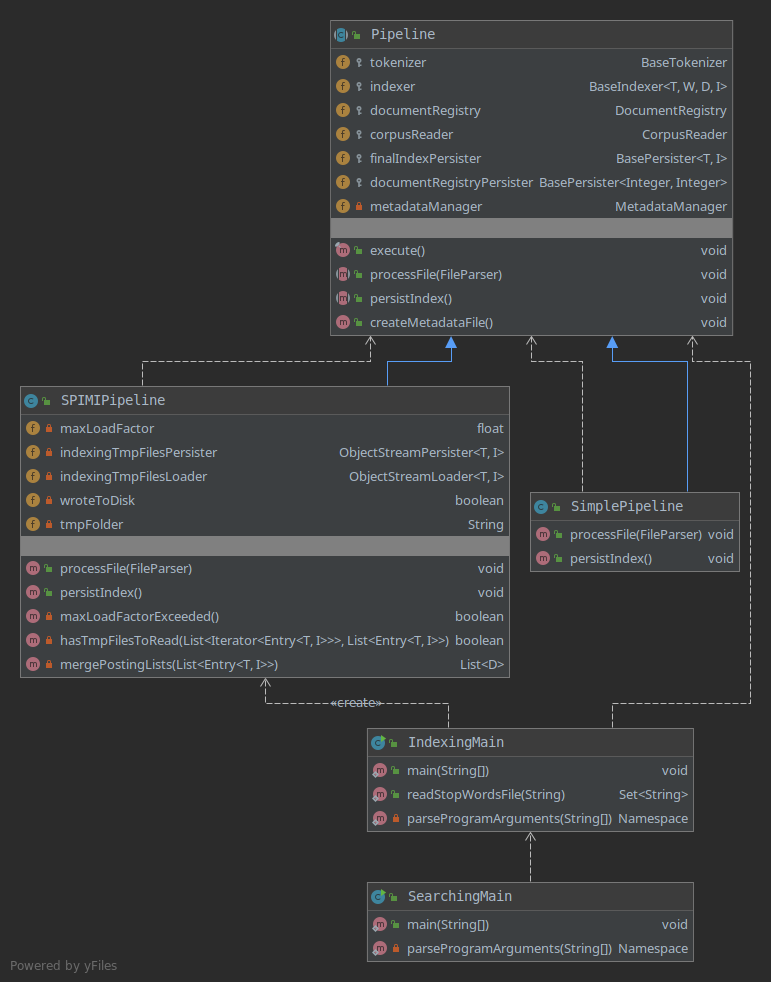
\includegraphics[width=10cm]{packages_mains.png}
  \caption{Diagrama de classes do package \it mains}
\end{figure}

Como agora temos de criar uma outra aplicação para procurar sobre os
indexers gerados, criamos um novo main em que executamos um conjunto
de queries recebidas de um ficheiro que são enviadas para o Search
sendo depois os resultados avaliados pela classe Evalutation.

\newpage

\section*{4. Resultados}

Resultados usando os dois ficheiro 2004\_TREC\_ASCII\_MEDLINE gz em
que as leituras a disco foram feitas sobre um HDD e o CPU i5-6300HQ
CPU @ 2.30GHz.

\begin{center}
    \small
    \begin{tabular}{| c | c | c | c | c | c |}
            \hline
            K
            & \bf  Média precision
            & \bf  Média recall
            & \bf  Média F-measure
            & \bf  Média Average Precision
            & \bf  Média NDCG \\ \hline

            10
            & 0.284
            & 0.064
            & 0.085
            & 0.429
            & 0.508 \\ \hline

            20
            & 0.242
            & 0.078
            & 0.100
            & 0.434
            & 0.529 \\ \hline

            50
            & 0.202
            & 0.111
            & 0.125
            & 0.390
            & 0.500 \\ \hline

    \end{tabular}
\end{center}

Foi feito também um estudo do impacto do tamanho dos ficheiros dos
segmentos do indexer e document registry na query latency e query
throughput.

Estes testes foram corridos dando à JVM o máximo de memória 2G.
O programa funciona para limites de memória mais baixos como por
exemplo 1G no entanto é preciso alterar algumas definições de defeito
definindo algumas opções do programa.

\begin{center}
    \small
    \begin{tabular}{| c | c | c |}
        \hline
        K
        & \bf Query latency (segundos)
        & \bf Query throughput (por segundo) \\ \hline

        \multicolumn{3}{|c|}{Indexer: 10MB, Document Registry: 25MB} \\ \hline

        10
        & 0.709
        & 1.411 \\ \hline

        20
        & 0.698
        & 1.433 \\ \hline

        50
        & 0.653
        & 1.531 \\ \hline

        \multicolumn{3}{|c|}{Indexer: 10MB, Document Registry: 50MB} \\ \hline

        10
        & 0.714
        & 1.400 \\ \hline

        20
        & 0.678
        & 1.474 \\ \hline

        50
        & 0.796
        & 1.256 \\ \hline

        \multicolumn{3}{|c|}{Indexer: 25MB, Document Registry: 25MB} \\ \hline

        10
        & 0.884
        & 1.131 \\ \hline

        20
        & 0.913
        & 1.096 \\ \hline

        50
        & 0.815
        & 1.227 \\ \hline

        \multicolumn{3}{|c|}{Indexer: 25MB, Document Registry: 50MB} \\ \hline

        10
        & 0.924
        & 1.083 \\ \hline

        20
        & 0.862
        & 1.161 \\ \hline

        50
        & 0.950
        & 1.053 \\ \hline

        \multicolumn{3}{|c|}{Indexer: 50MB, Document Registry: 25MB} \\ \hline

        10
        & 1.127
        & 0.887 \\ \hline

        20
        & 1.269
        & 0.788 \\ \hline

        50
        & 1.087
        & 0.920 \\ \hline

        \multicolumn{3}{|c|}{Indexer: 50MB, Document Registry: 50MB} \\ \hline

        10
        & 1.176
        & 0.850 \\ \hline

        20
        & 1.099
        & 0.910 \\ \hline

        50
        & 1.223
        & 0.818 \\ \hline

    \end{tabular}
\end{center}

De maneira a gerar os vários indexar o mais rápido, geramos um script
que lançava o processo de indexação com o máximo de memória
disponível (por volta de 6G) em que os tempos variaram entre 36
minutos e 60 minutos.

Podemos ver também que que os tempos melhoram com ficheiros com menos
tamanho no entanto isto pode levar a um grande número de segmentos,
tendo assim que ter mais metadados em memória.

\newpage

\section*{5. Anexos}

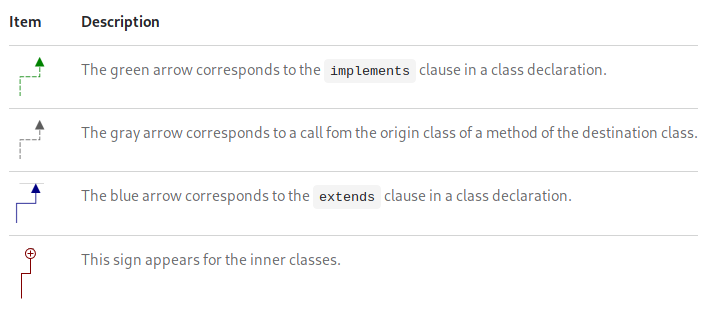
\includegraphics[width=13cm]{arrow_legend.png}

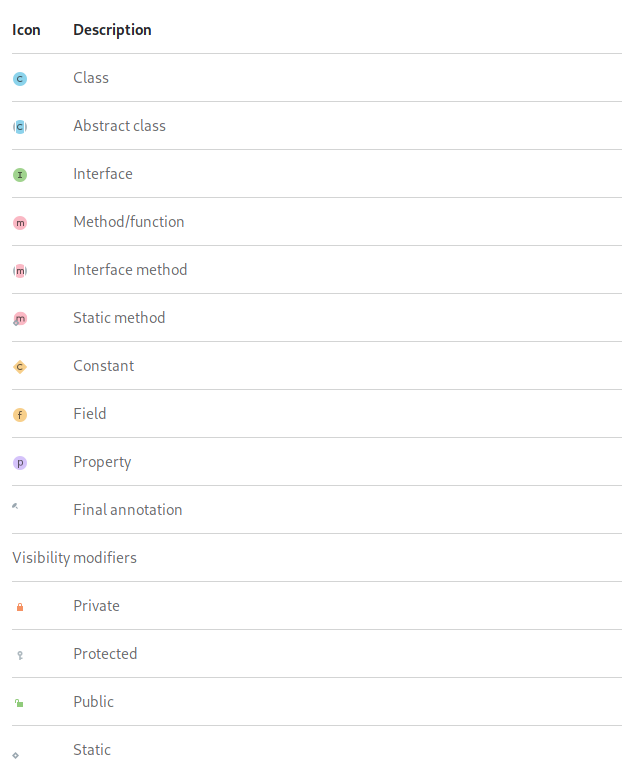
\includegraphics[width=13cm]{icons_legend.png}

\end{document}
